\documentclass[12pt]{report}
\usepackage[utf8]{inputenc}
\usepackage[T1]{fontenc}
\usepackage[french]{babel}
\usepackage{graphicx}
\usepackage{hyperref}
\usepackage{lmodern}
\usepackage{fancyhdr}
\usepackage{geometry}
\usepackage{float}


\geometry{margin=2.5cm}
\pagestyle{fancy}
\fancyhf{}
\rhead{\thepage}
\lhead{
\includegraphics[width=1.8cm]{Logo_nanterre.png}} % logo école en en-tête

% PAGE DE GARDE CUSTOM
\begin{document}

\begin{titlepage}
    \centering
    
\includegraphics[width=3.5cm]{Logo_nanterre.png}\par\vspace{1cm}
    {\scshape\LARGE Université Paris Nanterre\par}
    \vspace{0.5cm}
    {\huge\bfseries Rapport de Projet\par}
    \vspace{0.5cm}
    {\Huge\bfseries AutoPredict\par}
    \vspace{1.5cm}
    {\Large \textbf{Membres du projet :} \par}
    \vspace{0.3cm}
    {\Large X. Frédéric \\ R. Yann \\ R. Jérémy \par}
    \vfill
    {\large \today\par}
\end{titlepage}

\tableofcontents

\chapter{Présentation de AutoPredict}
\section{Problématique}
Le choix d’une voiture peut s’avérer complexe pour un acheteur, en particulier lorsque de nombreux critères entrent en jeu : budget, type de motorisation, consommation, puissance, style, marque, etc. Les plateformes existantes n’offrent pas toujours une expérience personnalisée ou intuitive pour explorer l’offre de véhicules selon ses préférences réelles. Par ailleurs, les vendeurs ou les analystes souhaitent mieux comprendre les facteurs qui influencent le prix d’un véhicule, et optimiser leur stratégie de vente.


\section{Solution}
AutoPredict est une plateforme web intelligente permettant d’exploiter une base de données automobile pour proposer deux fonctionnalités principales :

\begin{itemize}
    \item \textbf{Recherche assistée de modèles} : à partir d’un budget donné et de certaines préférences (ex. type de transmission, puissance, taille...), l’utilisateur reçoit une liste de véhicules correspondant à ses besoins.
    \item \textbf{Estimation de prix} : à partir des caractéristiques sélectionnées (ex. année, style, consommation...), l’utilisateur obtient une estimation de la fourchette de prix des véhicules correspondants.
\end{itemize}

Ces fonctionnalités sont rendues possibles grâce à une architecture combinant analyse de données, machine learning, backend intelligent et une interface frontend intuitive.


\chapter{Caractéristiques Principales}
\section{Interface Conviviale}
L’interface utilisateur est conçue avec ReactJS pour offrir une navigation fluide et interactive.
L’accent est mis sur l’ergonomie, la clarté des résultats et la facilité d’utilisation même pour des utilisateurs non-experts.


\section{Sources Fiables}
Les données utilisées proviennent de datasets publics sur les voitures, incluant des caractéristiques techniques (puissance, consommation, taille, style), économiques (prix, popularité), et temporelles (année de sortie).

\chapter{Architecture métier}
\section{Frontend}
Le frontend est développé en ReactJS. Il intègre des composants interactifs permettant à l’utilisateur de :

\begin{itemize}
    \item Rechercher des modèles de voitures correspondant à ses critères et à son budget
    \item Estimer la valeur d’un véhicule en fonction de caractéristiques spécifiques
    \item Visualiser graphiquement les résultats obtenus (filtres, comparateurs, graphiques de prix, etc.)
\end{itemize}

L’interface dialogue avec le backend via une API REST.


\section{Backend}
Le backend est conçu en Python à l’aide du framework Flask. Il gère :

\begin{itemize}
    \item L’accès à la base NoSQL contenant les données automobiles
    \item L’exécution des modèles de machine learning pour la recommandation de véhicules et l’estimation des prix
    \item L’interface avec le frontend via une API structurée
\end{itemize}

Les requêtes utilisateurs sont traitées dynamiquement pour retourner des résultats adaptés et rapides.


\section{Base de données}
La base de données utilisée est de type NoSQL, permettant une flexibilité dans la gestion des formats de données hétérogènes typiques du domaine automobile.

\chapter{Architecture distribuée}
\section{Application Hosting}
Le projet est conteneurisé afin de faciliter le déploiement, la scalabilité et la portabilité. Docker est utilisé pour packager les composants.

\section{Database Hosting}
La base NoSQL est hébergée dans un environnement compatible cloud. Elle stocke les jeux de données enrichis et traités, accessibles via API.

\chapter{Pratiques de Collaboration et de DevOps}
\section{Project Management}
Le projet est géré en équipe de trois membres : Frédéric, Yann et Jérémy. Le suivi des tâches se fait de manière collaborative autour d'outils de gestion agile.

\section{Versionnement}
L’ensemble du code source est versionné via Git, avec des dépôts organisés pour le frontend, le backend et les notebooks d'analyse/ML.

\section{Intégration Continue et Déploiement Continu}
Des pipelines CI/CD seront mis en place pour automatiser les tests, le linting, et le déploiement sur l’environnement de développement.

\section{Maintenabilité du code}
L'utilisation de conteneurs, de frameworks standards (Flask, React) et de pratiques de développement modulaire assure la maintenabilité du projet.

\section{Qualité du code}
Le code est documenté, typé et validé avec des outils de linting et des tests unitaires, notamment sur les scripts de preprocessing et les modèles ML.

\chapter{Partie Data Analytique}

\thispagestyle{plain}
\pagestyle{plain}


\section{Analyse de données}

\subsection{Préparation et nettoyage des données}

La phase de préparation a consisté à rendre les données cohérentes, complètes et prêtes à être visualisées. Elle s’est déroulée comme suit :

\begin{itemize}
  \item \textbf{Standardisation} : Uniformisation des noms de colonnes en minuscules avec des underscores pour assurer une manipulation fluide.
  \item \textbf{Suppression des doublons} : Élimination des entrées redondantes basées sur les identifiants véhicule/modèle.
  \item \textbf{Traitement des valeurs manquantes} :
    \begin{itemize}
        \item Remplacement par des valeurs par défaut ou par la moyenne (ex. nombre de portes ou de cylindres).
        \item Suppression des lignes avec des données critiques absentes.
    \end{itemize}
  \item \textbf{Filtrage des transmissions inconnues} : Les entrées comportant `UNKNOWN` pour la transmission ont été exclues de l’analyse.
  \item \textbf{Création de nouvelles variables} :
    \begin{itemize}
        \item Quantiles de prix (MSRP) pour catégoriser les véhicules.
        \item Plages de puissance moteur pour les regrouper en catégories (`faible`, `moyenne`, `élevée`, etc.).
        \item Calcul de la consommation moyenne combinée (ville + autoroute).
    \end{itemize}
\end{itemize}

\subsection{Présentation des graphiques et interprétation}

Dans cette section, nous explorons différentes visualisations de données afin d’extraire des tendances structurelles sur notre flotte de véhicules. Chaque graphique est accompagné d’une interprétation opérationnelle, utile pour guider les recommandations clients.

\paragraph{1. Répartition des types de transmission selon les quantiles de prix}\mbox{}

\begin{figure}[H]
\centering
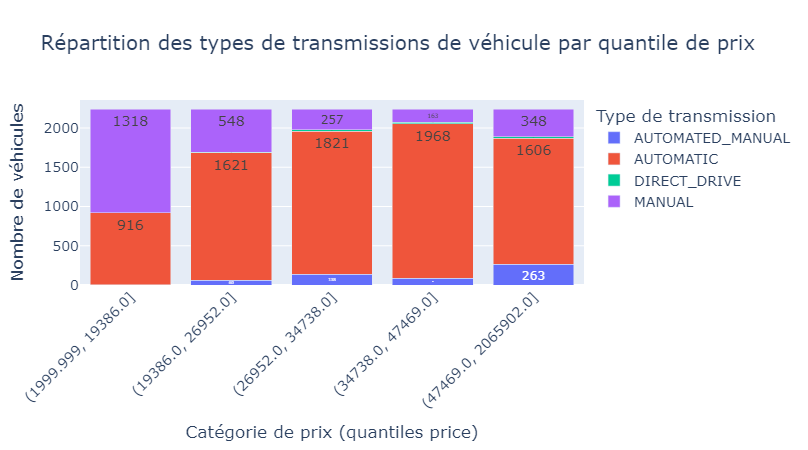
\includegraphics[width=0.8\textwidth]{transmission_vs_price.png}
\caption{Répartition des transmissions par tranche de prix (quantiles MSRP)}
\end{figure}


Ce graphique à barres empilées montre que :
\begin{itemize}
  \item Les transmissions \textbf{automatiques} dominent très largement dans les gammes de prix \textit{intermédiaires à élevées}, représentant parfois plus de \textbf{80 \%} des véhicules.
  \item Les transmissions \textbf{manuelles} sont surtout présentes dans les véhicules du \textit{premier quantile de prix}, et disparaissent progressivement à mesure que le prix augmente.
  \item Les transmissions \textbf{automatisées manuelles} sont rares, présentes essentiellement dans des véhicules haut de gamme ou spécifiques.
\end{itemize}

Cette distribution illustre un lien direct entre la gamme tarifaire et le type de confort/conduite attendu.

\paragraph{2. Répartition des styles de véhicules selon le type de transmission}\mbox{}

\begin{figure}[H]
\centering
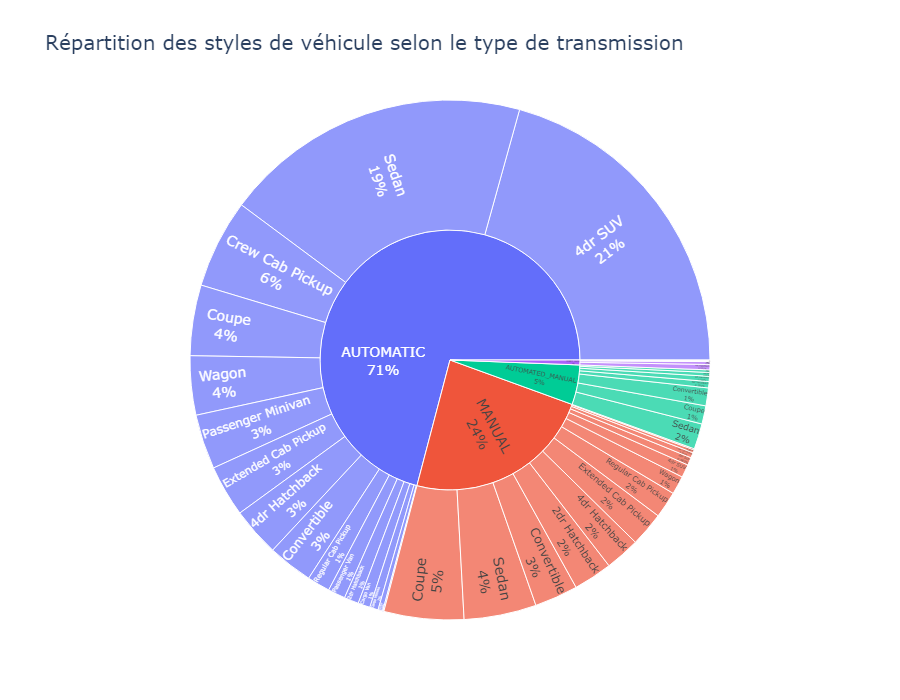
\includegraphics[width=0.8\textwidth]{transmission_style_sunburst.png}
\caption{Répartition des styles de véhicule selon la transmission}
\end{figure}

Le diagramme sunburst confirme les tendances précédentes :
\begin{itemize}
  \item Les \textbf{SUV} et \textbf{berlines (sedan)} sont principalement associés aux transmissions automatiques, répondant à des besoins de confort et d’usage urbain/familial.
  \item Les \textbf{coupés}, \textbf{hatchbacks} ou \textbf{pickups} sont souvent en transmission manuelle, adaptés à des usages économiques, sportifs ou professionnels.
  \item Les transmissions rares comme \texttt{DIRECT\_DRIVE} restent anecdotiques.
\end{itemize}

\paragraph{3. Consommation moyenne selon puissance moteur et cylindres}\mbox{}

\begin{figure}[H]
\centering
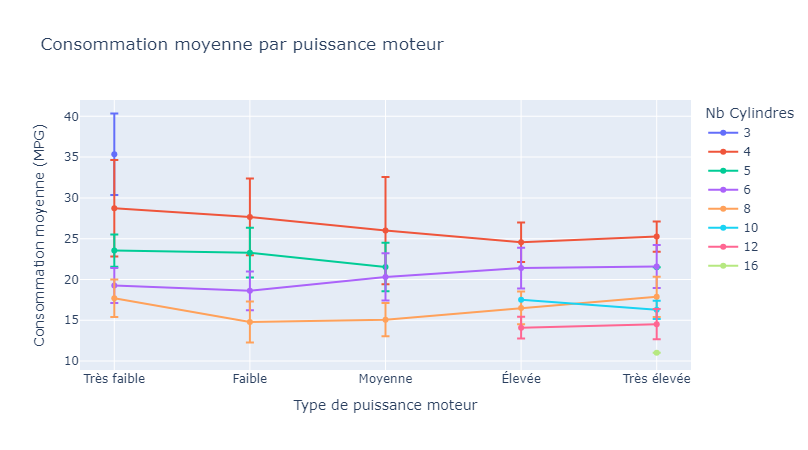
\includegraphics[width=0.8\textwidth]{hp_vs_cylinders.png}
\caption{Consommation moyenne selon puissance moteur et nombre de cylindres}
\end{figure}

On observe une relation logique entre la puissance du moteur et la consommation :
\begin{itemize}
  \item Les véhicules à \textbf{puissance très élevée} et \textbf{8 cylindres ou plus} affichent une consommation moyenne plus élevée.
  \item Les modèles à \textbf{puissance moyenne à faible} ont des consommations plus stables et optimisées.
  \item Cette analyse permet de recommander les modèles selon un compromis performance/efficacité.
\end{itemize}

\paragraph{4. Prix moyen par catégorie de véhicule et puissance moteur}\mbox{}

\begin{figure}[H]
\centering
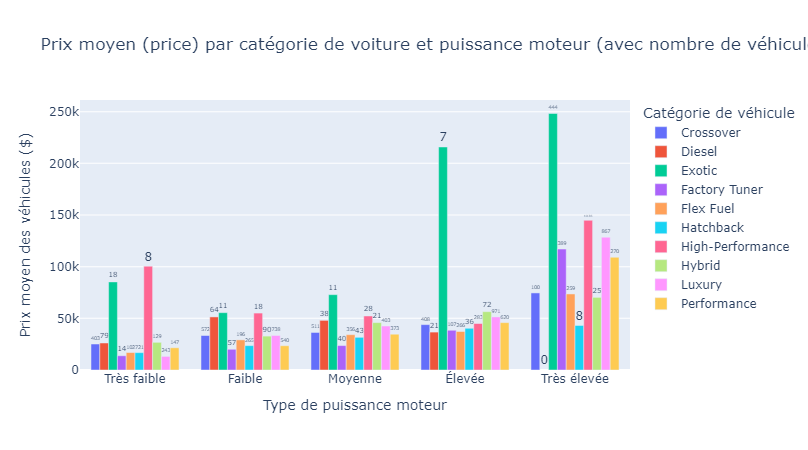
\includegraphics[width=0.9\textwidth]{price_vs_hp_market.png}
\caption{Prix moyen par catégorie de voiture et puissance moteur (avec nombre de véhicules)}
\end{figure}

Cette visualisation en barres groupées révèle :
\begin{itemize}
  \item Les véhicules \textbf{exotiques} dominent dans les plages de puissance élevée avec un prix moyen largement supérieur à 200 000\$.
  \item La catégorie \textbf{haut de gamme (Luxury)} est répartie sur toutes les puissances, mais fortement concentrée sur les plages hautes.
  \item Les \textbf{véhicules hybrides, diesel, flex fuel} et \textbf{compactes (Hatchback)} occupent les plages basses à moyennes, avec des prix accessibles.
\end{itemize}

Ce graphique complète la compréhension des segments en croisant l’offre produit avec les puissances moteur disponibles.

\paragraph{5. Profil d’achat et recommandations commerciales}\mbox{}

\vspace{0.5cm}

À partir de l’ensemble de ces analyses, plusieurs profils-types émergent :
\begin{itemize}
  \item Un \textbf{client urbain familial}, à la recherche de confort et de fiabilité, sera orienté vers un \textbf{SUV automatique} de gamme intermédiaire.
  \item Un \textbf{client professionnel ou rural} peut viser un \textbf{pickup manuel}, robuste et économique.
  \item Un \textbf{jeune conducteur ou petit budget} sera conseillé vers un \textbf{coupé ou hatchback manuel}, situé dans les premiers quantiles de prix.
  \item Pour les \textbf{amateurs de performance ou de véhicules hybrides}, on oriente vers des modèles à forte puissance ou technologies spécifiques, tout en tenant compte du marché (exotic, performance, luxury).
\end{itemize}

L’approche analytique appliquée à nos données permet donc d’alimenter directement notre moteur de recommandation personnalisé.


\subsection{Analyse de la diversification de marque et de modèle}
\begin{figure}[H]
    \centering
    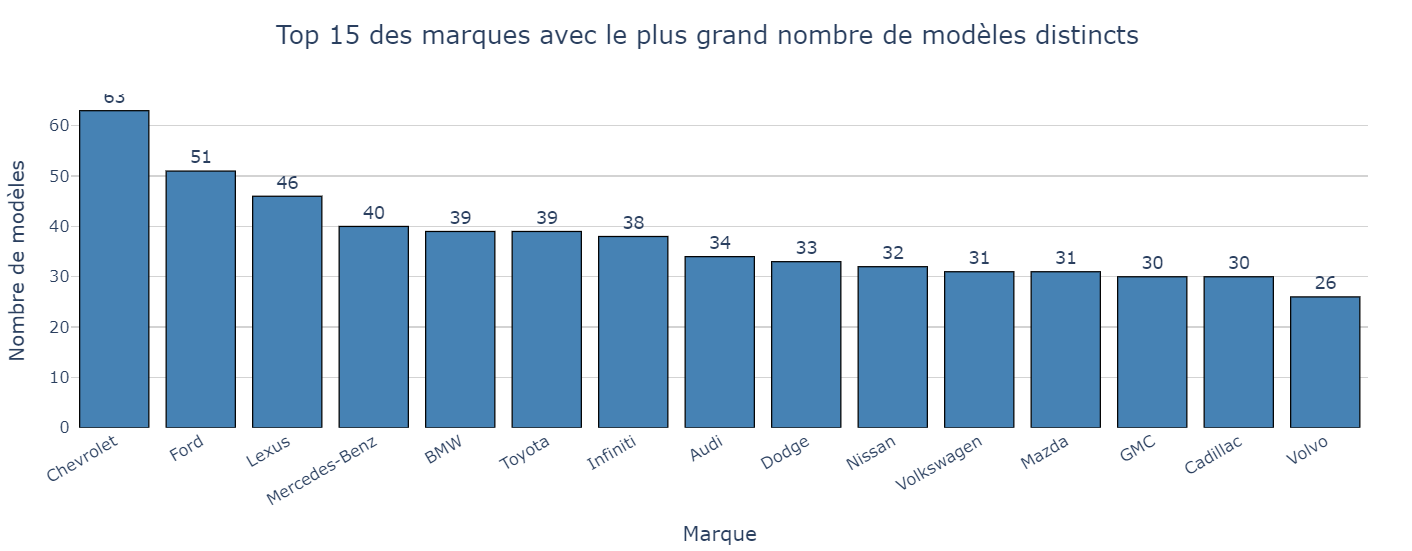
\includegraphics[width=1\textwidth]{Modele_marque.png}
    \caption{Top 15 des marques avec le plus grand nombre de modèles distincts}
    \label{fig:modele-marque}
\end{figure}

Ce graphique met en évidence les marques proposant le plus grand nombre de modèles différents. \textbf{Chevrolet} et \textbf{Ford} occupent les premières places avec respectivement 63 et 51 modèles, témoignant d’une stratégie de gamme très étendue. D’autres marques comme \textbf{Lexus}, \textbf{Mercedes-Benz} ou \textbf{BMW} offrent également un catalogue riche, mais plus orienté haut de gamme. Ce volume important de modèles suggère une forte présence sur le marché et une capacité à répondre à des profils variés de clients.


\begin{figure}[H]
    \centering
    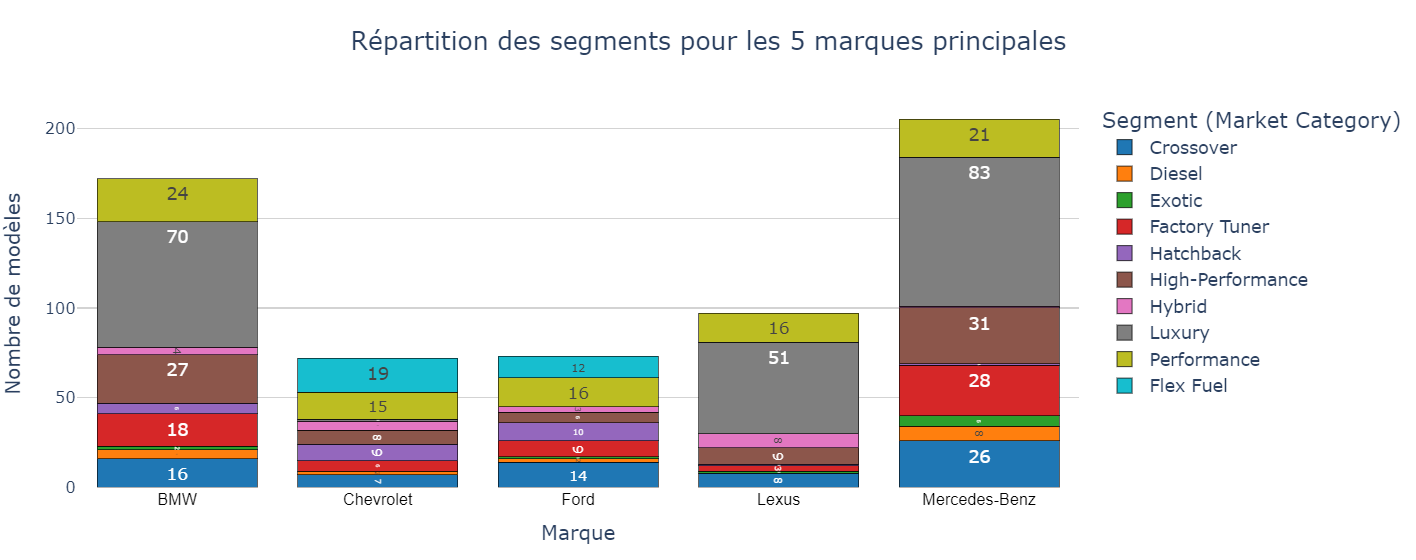
\includegraphics[width=1\textwidth]{Marque_nbmodele.png}
    \caption{Répartition des segments pour les 5 marques principales}
    \label{fig:marque-nbmodele}
\end{figure}

\vspace{1em}
\textbf{Observations principales}
\begin{itemize}
    \item \textbf{BMW} et \textbf{Mercedes-Benz} se distinguent par une forte concentration de modèles dans le segment \textit{Luxury}, avec respectivement 70 et 83 modèles.
    \item \textbf{Mercedes-Benz} est la marque la plus segmentée, avec des modèles présents dans presque toutes les catégories : Crossover, Performance, Factory Tuner, etc.
    \item \textbf{Chevrolet} et \textbf{Ford} affichent une répartition plus équilibrée entre les segments, bien que moins dense en nombre total.
    \item \textbf{Lexus} adopte une stratégie proche de Mercedes-Benz, mais dans une échelle plus réduite : forte présence sur le \textit{Luxury}, accompagnée de quelques modèles Performance, Hybrid et Crossover.
\end{itemize}

\vspace{1em}
\textbf{Points clés à retenir}
\begin{itemize}
    \item Les marques comme \textbf{BMW} et \textbf{Mercedes-Benz} ciblent principalement le haut de gamme avec une concentration marquée sur le segment \textit{Luxury}.
    \item \textbf{Mercedes-Benz} se distingue par une couverture quasi complète des segments, traduisant une stratégie premium mais aussi étendue.
    \item \textbf{Ford} et \textbf{Chevrolet} privilégient une stratégie généraliste, en diversifiant leurs modèles sur différents segments.
    \item \textbf{Lexus} suit un modèle proche de Mercedes-Benz, mais avec un catalogue plus restreint.
\end{itemize}

\vspace{1em}
\textbf{Implications pour AutoPredict}

\begin{itemize}
    \item Les marques aux offres diversifiées sont pertinentes pour répondre à différents profils clients et alimenter des recommandations plus personnalisées.
    \item Les marques spécialisées peuvent mieux correspondre à des besoins ciblés ou des utilisateurs ayant des préférences affirmées.
    \item Ces données enrichissent notre moteur de suggestion, en affinant les correspondances entre segments de véhicules et attentes utilisateurs (prix, performance, consommation, etc.).
\end{itemize}

\begin{figure}[H]
    \centering
    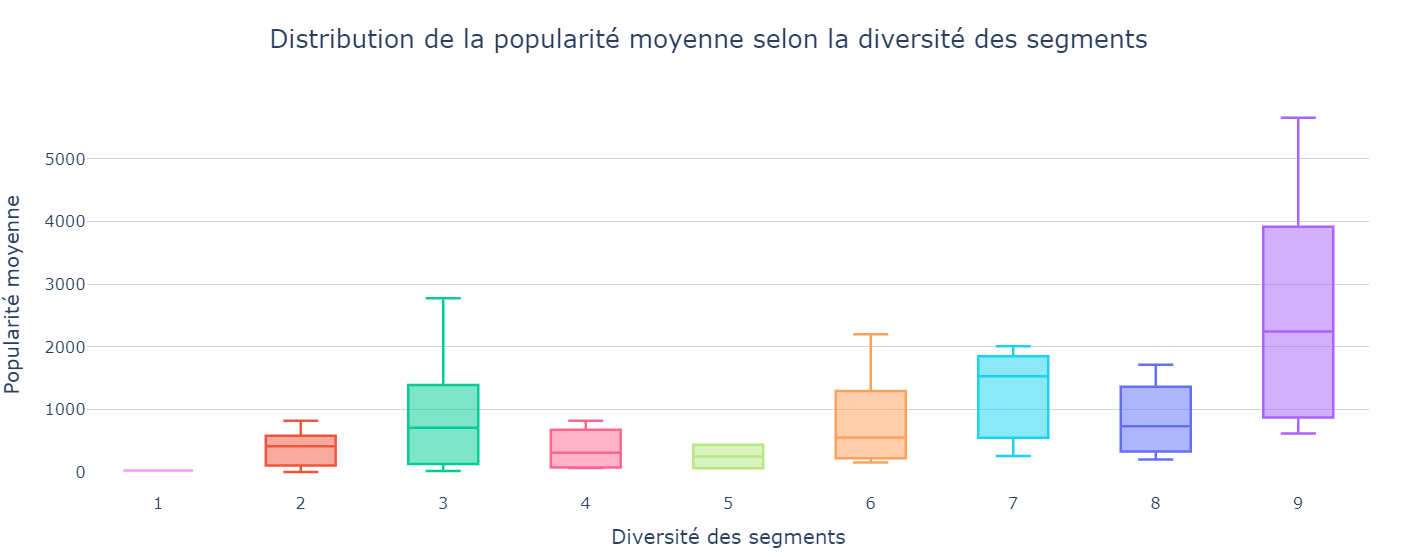
\includegraphics[width=1\textwidth]{Section_pop.png}
    \caption{Distribution de la popularité moyenne selon la diversité des segments}
    \label{fig:section-pop}
\end{figure}


L’analyse de la relation entre le nombre de segments couverts par une marque et sa popularité moyenne révèle une tendance globale : les marques les plus populaires sont souvent celles dont l’offre est la plus diversifiée.

Les marques couvrant peu de segments (1 à 3) restent relativement peu visibles, tandis que celles qui atteignent une couverture large (8 à 9 segments) bénéficient en moyenne d’un niveau de popularité plus élevé. Cette observation suggère qu’une stratégie de diversification permet de mieux répondre à la variété des attentes des clients et d’élargir la portée commerciale d’une marque.

Toutefois, cette tendance s’accompagne d’une forte dispersion : certaines marques très diversifiées restent peu populaires, tandis que d’autres, bien que spécialisées, conservent une forte notoriété. Cela montre que la diversité ne suffit pas à elle seule : l’image de marque, le positionnement marketing et la perception client jouent un rôle tout aussi déterminant.

En résumé, la diversité de l’offre constitue un levier important dans la construction d’une marque attractive. Pour AutoPredict, cet indicateur peut être intégré au moteur de recommandation pour ajuster les propositions en fonction de la stratégie produit des constructeurs et du profil de l’utilisateur.


\subsection{Analyse de la dépréciation}

\begin{figure}[H]
    \centering
    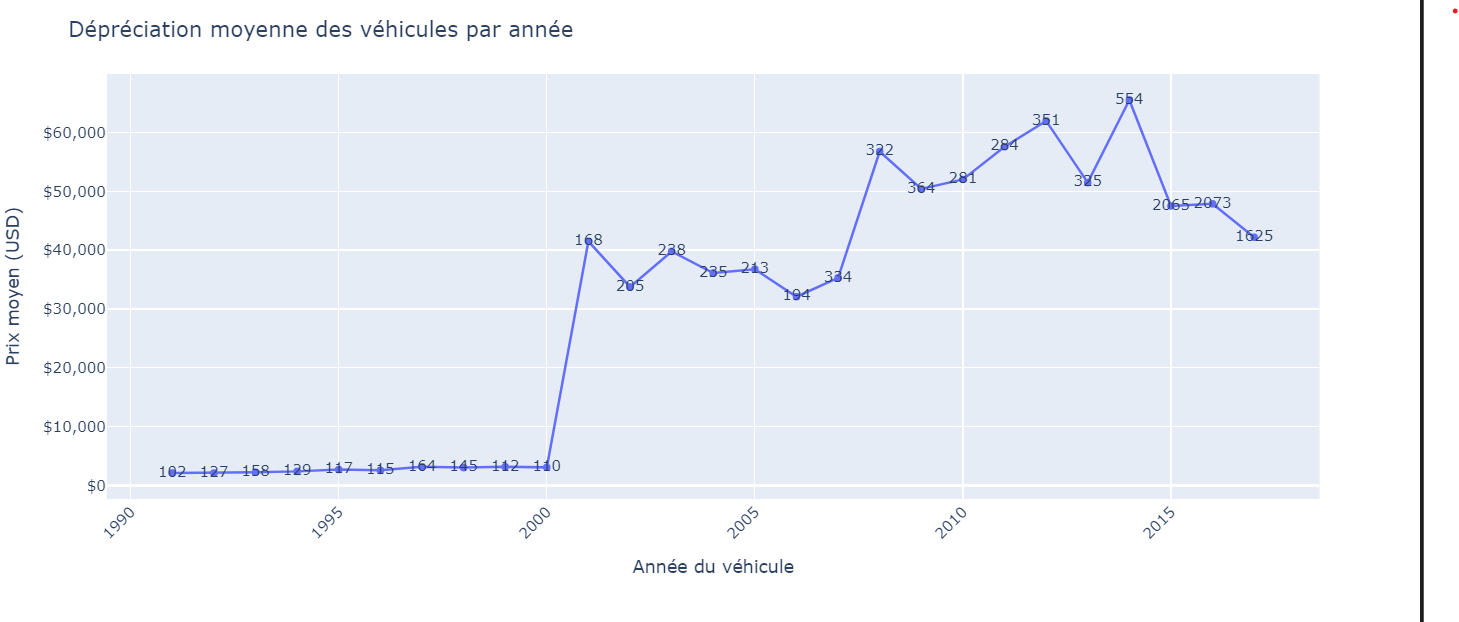
\includegraphics[width=1\textwidth]{Annee_prix.png}
    \caption{Dépréciation moyenne des véhicules pas année}
    \label{fig:annee-prix}
\end{figure}

Cette visualisation offre une vue d’ensemble de l’évolution du prix moyen des véhicules selon leur année de fabrication, sur un marché combinant véhicules neufs et d’occasion.

On observe une baisse marquée des prix pour les véhicules produits entre 1990 et 1999, souvent vendus sous la barre des 10 000 dollars. Entre 2000 et 2002, une chute brutale est visible, possiblement liée à l’impact de nouvelles normes environnementales pénalisant les véhicules plus anciens.

À partir de 2005, la courbe devient plus régulière et progresse graduellement jusqu’à atteindre environ 37 000 dollars en 2017. Cette évolution reflète une montée en gamme progressive des véhicules récents, tant en termes de technologie que de confort ou de positionnement commercial.

Dans l’ensemble, les données révèlent une dépréciation rapide des véhicules au cours de leurs 10 à 15 premières années. Un véhicule de plus de 15 ans perd une part importante de sa valeur, ce qui limite sa rentabilité en revente.

\vspace{1em}
Cette première analyse met en lumière la tendance générale du marché. Elle soulève toutefois une interrogation essentielle : tous les styles de véhicules suivent-ils cette même trajectoire de dépréciation ? C’est à cette question que nous répondrons dans la section suivante.


\begin{figure}[H]
    \centering
    \includegraphics[width=1\textwidth]{année_pris_dep.png}
    \caption{Dépréciation par style de véhicule}
    \label{fig:annee-pris-dep}  
\end{figure}

Cette analyse explore l’impact du style de carrosserie sur la dépréciation des véhicules au fil du temps. Chaque courbe du graphique représente un type de véhicule, avec en ordonnée le prix moyen par année de mise en circulation.

\vspace{0.5em}
\textbf{Observations notables :}
\begin{itemize}
    \item Les SUV 4 portes, Convertibles et Crew Cab Pickups conservent des prix élevés, même plusieurs années après leur sortie, ce qui reflète une forte demande et une bonne rétention de valeur.
    \item À l’inverse, les Cargo Vans, Hatchbacks 2 portes et Sedans affichent des prix plus faibles, même pour des modèles récents, traduisant une faible valorisation sur le marché secondaire.
    \item Les Convertible SUV, bien que rares, se distinguent par une valeur très élevée, probablement liée à leur rareté et à leur positionnement haut de gamme.
\end{itemize}

\vspace{0.5em}
\textbf{Interprétation générale :}
\begin{itemize}
    \item Les styles utilitaires ou économiques ont tendance à perdre rapidement de la valeur.
    \item Les styles plaisir ou valorisants (SUV, convertible, pickup) maintiennent mieux leur prix avec le temps.
    \item Passé 15 ans, la plupart des véhicules, quel que soit leur style, tendent vers une valeur moyenne d’environ 10 000 dollars.
\end{itemize}

\vspace{1em}
Le style du véhicule, en tant que facteur esthétique et fonctionnel, influence directement sa perception et sa valeur résiduelle. Toutefois, cette dimension visuelle s’inscrit aussi dans une stratégie de positionnement marketing, que nous approfondissons dans la prochaine section à travers l’analyse des catégories de marché.


\begin{figure}[H]
    \centering
    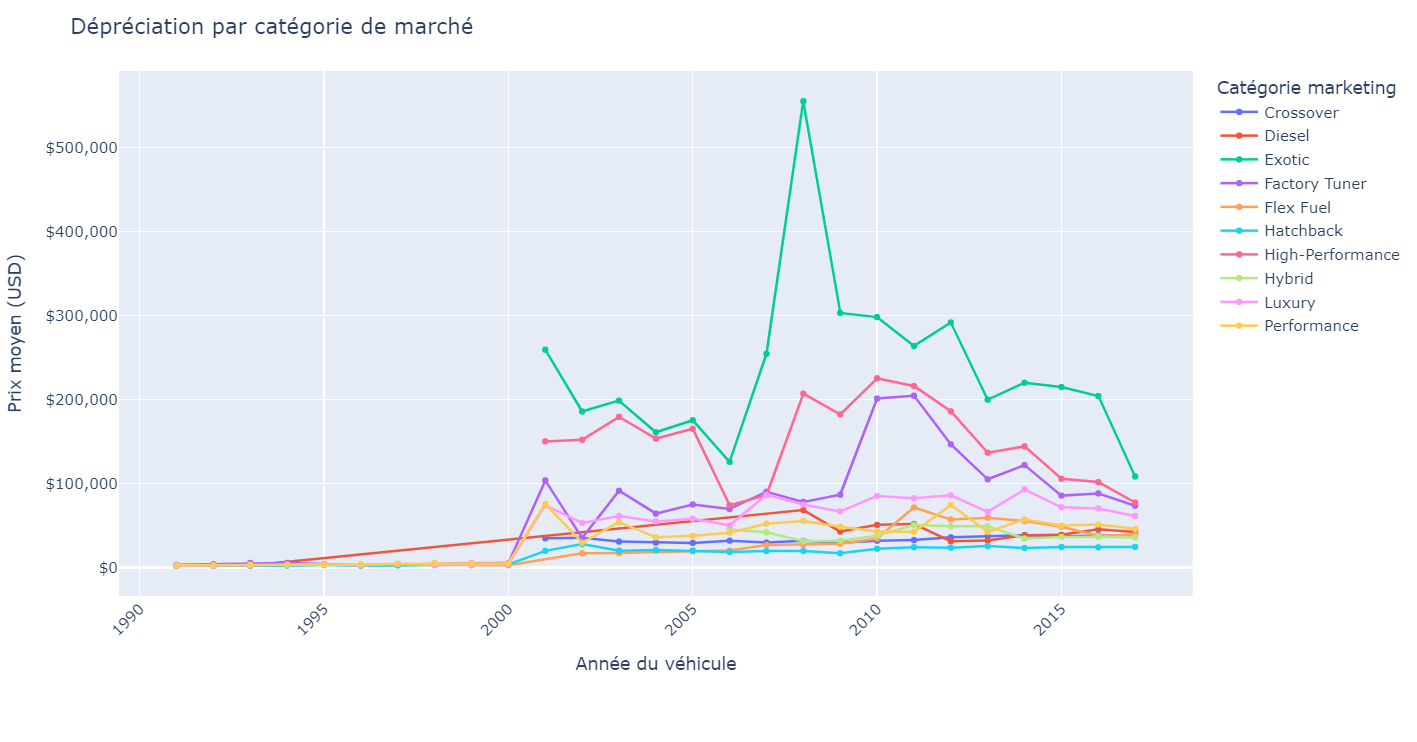
\includegraphics[width=1\textwidth]{annee_prix_cat.png}
    \caption{Dépréciation par catégorie de marché}
    \label{fig:annee-prix-cat}
\end{figure}
Cette analyse s’intéresse à la relation entre le positionnement commercial des véhicules (catégorie marketing) et leur maintien de valeur au fil du temps. Les catégories correspondent à des segments tels que \textit{Luxury}, \textit{Hybrid}, \textit{Diesel}, etc., qui traduisent une stratégie de marque ciblée.

\vspace{0.5em}
\textbf{Observations clés :}
\begin{itemize}
    \item Les segments \textit{Exotic}, \textit{High-Performance} et \textit{Luxury} dominent largement, avec des prix moyens dépassant fréquemment les 60 000 dollars, y compris pour des véhicules de 5 à 10 ans.
    \item Les catégories comme \textit{Diesel}, \textit{Hatchback} ou \textit{Flex Fuel} restent bien en dessous de la barre des 30 000 dollars. Ces modèles économiques ou écologiques subissent une dépréciation plus rapide.
    \item Le segment \textit{Crossover} montre une très bonne tenue de valeur, en combinant confort, modernité et polyvalence, ce qui en fait un choix populaire et stratégique.
\end{itemize}

\vspace{0.5em}
\textbf{Interprétation globale :}
\begin{itemize}
    \item La catégorie marketing influence fortement la rétention de valeur : les modèles haut de gamme, performants ou hybrides sont mieux valorisés dans le temps.
    \item À l’inverse, les véhicules à vocation pratique ou économique, bien qu’utiles, perdent plus rapidement de leur valeur.
\end{itemize}

\vspace{1em}
Ces résultats confirment que la perception du véhicule joue un rôle central dans sa valeur résiduelle. Intégrer cette information dans le moteur de recommandation d'AutoPredict permet d’adapter les suggestions aux attentes des utilisateurs, en tenant compte de leur sensibilité au prestige, à la performance ou à l’économie.

\end{document}
